\section{Gravity waves}
\label{sec:gw}

\TODO{introduce the test, justify its purpose}

\subsection{Specification}
Following \textcite{melvin2010}, the domain is \SI{300}{\kilo\meter} wide and \SI{30}{\kilo\meter} high.  The mountain profile has the same form as equation~\ref{eqn:resting:mountain} but with a lower maximum height of $\surface_0 = \SI{250}{\meter}$.  As in the resting atmosphere test, $a = \SI{5}{\kilo\meter}$ is the mountain half-width and $\lambda = \SI{4}{\kilo\meter}$ is the wavelength.  On the optimised SLEVE grid, $s_1 = \SI{5}{\kilo\meter}$ is the large scale height, $s_2 = \SI{2}{\kilo\meter}$ is the small scale height and the optimal exponent value $n = 1.35$ as in the previous test\TODOsidenote{where did these SLEVE parameters come from?}.

The initial thermodynamic conditions have a surface temperature of $\theta_0 = \SI{288}{\kelvin}$ and constant stability with $N = \SI{0.01}{\per\second}$ everywhere.  A constant horizontal wind $u = \SI{10}{\meter\per\second}$ is prescribed at the inlet boundary.

\subsection{Discretisation}
The test uses the discretisation of the Euler equations described in section~\ref{sec:method:discretisation}.  The domain is discretised on a grid having $600 \times 100$ cells such that $\Delta x = \SI{0.5}{\kilo\meter}$ and $\Delta z = \SI{300}{\meter}$.  Sponge layers are added to the upper \SI{10}{\kilo\meter} and leftmost \SI{10}{\kilo\meter} at the inlet boundary to damp the reflection of waves.
The term $\mu \rho \vect{u}$ is subtracted from the momentum equation (equation~\ref{eqn:method:momentum}) where the damping function $\mu$ is adapted from \textcite{melvin2010} such that
\begin{align}
	\mu(x, z) &= \mu_\mathrm{upper} + \mu_\mathrm{inlet} \\
	\mu_\mathrm{upper}(z) &= \begin{cases}
		\overline{\mu} \sin^2 \left( \frac{\pi}{2} \frac{z - z_B}{H - z_B} \right) & \text{if } z \geq z_B \\
		0 & \text{otherwise} \\
	\end{cases} \\
	\mu_\mathrm{inlet}(x) &= \begin{cases}
		\overline{\mu} \sin^2 \left( \frac{\pi}{2} \frac{x_I - x}{x_I - x_0} \right) & \text{if } x < x_I \\
		0 & \text{otherwise}
	\end{cases}
\end{align}
where $\overline{\mu} = 1.2$ is the damping coefficient, $z_B = \SI{20}{\kilo\meter}$ is the bottom of the sponge layer, $H = \SI{30}{\kilo\meter}$ is the top of the domain, $x_0 = \SI{-150}{\kilo\meter}$ is the leftmost limit of the domain and $x_I = \SI{-140}{\kilo\meter}$ is the rightmost extent of the inlet sponge layer.  Note that, while the domain itself is \SI{30}{\kilo\meter} in height, for the purposes of generating of BTF and SLEVE grids, the domain height is set to \SI{20}{\kilo\meter} because the sponge layer occupies the uppermost \SI{10}{\kilo\meter}.

No slip conditions are imposed on the top and bottom boundaries and the outlet is zero gradient.  For Exner, hydrostatic balance is prescribed on all boundaries.  The simulation is integrated forward by 5 hours with a timestep $\Delta t = \SI{8}{\second}$.

\subsection{Results}

\TODO{compare with Melvin 2010?}

\hrule

\begin{itemize}
\item Reproduced result for BTF from W\&S
\item Vertical mixing at ground in lee of orography seen in results for snapCol and snap meshes.  This occurs in the lowest two rows of the mesh: lower layer $\theta$ is warmer, next layer above is cooler.  Feature is visible after t=3600s (Figure~\ref{fig:gw:mixing-3600s}), becomes more pronounced by t=18000s (Figure~\ref{fig:gw:mixing-18000s}).
\end{itemize}

\subsection{Investigation of vertical mixing}
Initially suspected mixing was due to computation mode of Lorenz vertical staggering but now it seems not:
\begin{itemize}
	\item plot UfDiff as a vector field doesn't seem to show any velocity anomalies in BTF or snalCol (Figure~\ref{fig:gw:ufdiff})
	\item plot of $\theta$ field shows that mixing is not strong enough to overcome stratification (Figure~\ref{fig:gw:theta})
	\item doubling mountain height causes mixing to appear in BTF case, and increases to three rows of mixing in SnapCol (Figure~\ref{fig:gw:double-height})
	\item halving $\Delta z$ also causes BTF mixing but less severe, also three rows of mixing in SnapCol (not shown)
	\item the results for dp/dx show mixing in BTF, and increased mixing in SnapCol (not shown)
\end{itemize}

\begin{figure}
	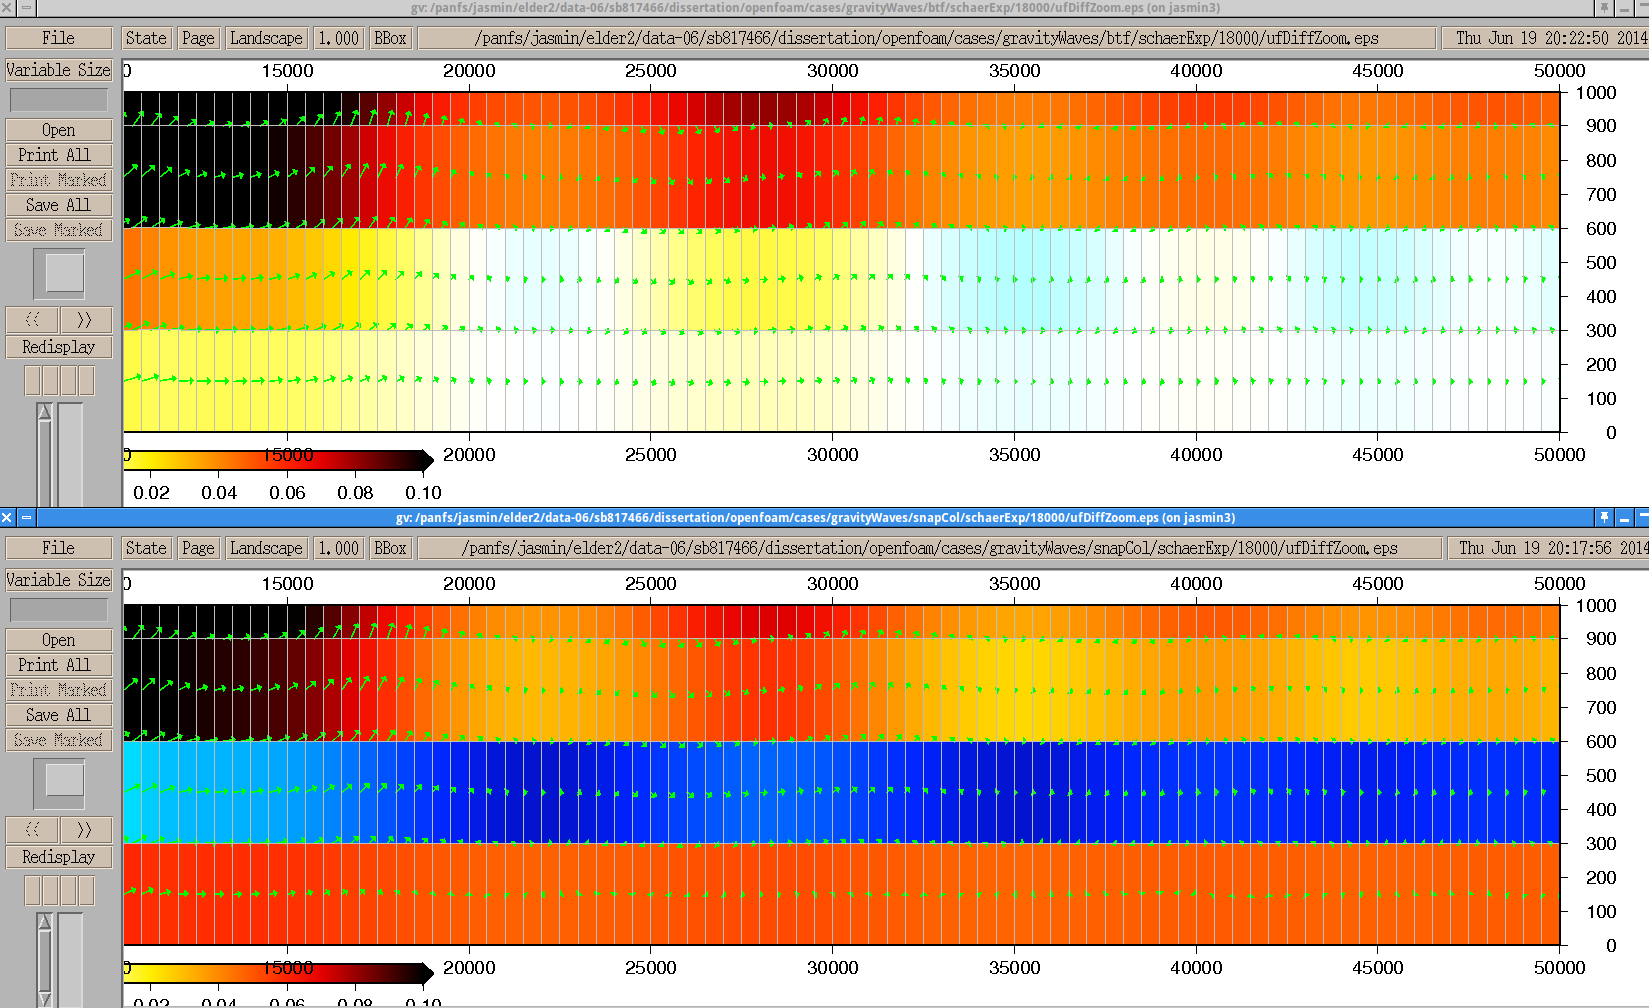
\includegraphics[width=\textwidth]{interim-results/gravityWavesBTFSnapColVelocityVectors.png}
	\caption{UfDiff after t=18000s, BTF and SnapCol meshes}
	\label{fig:gw:ufdiff}
\end{figure}

\begin{figure}
	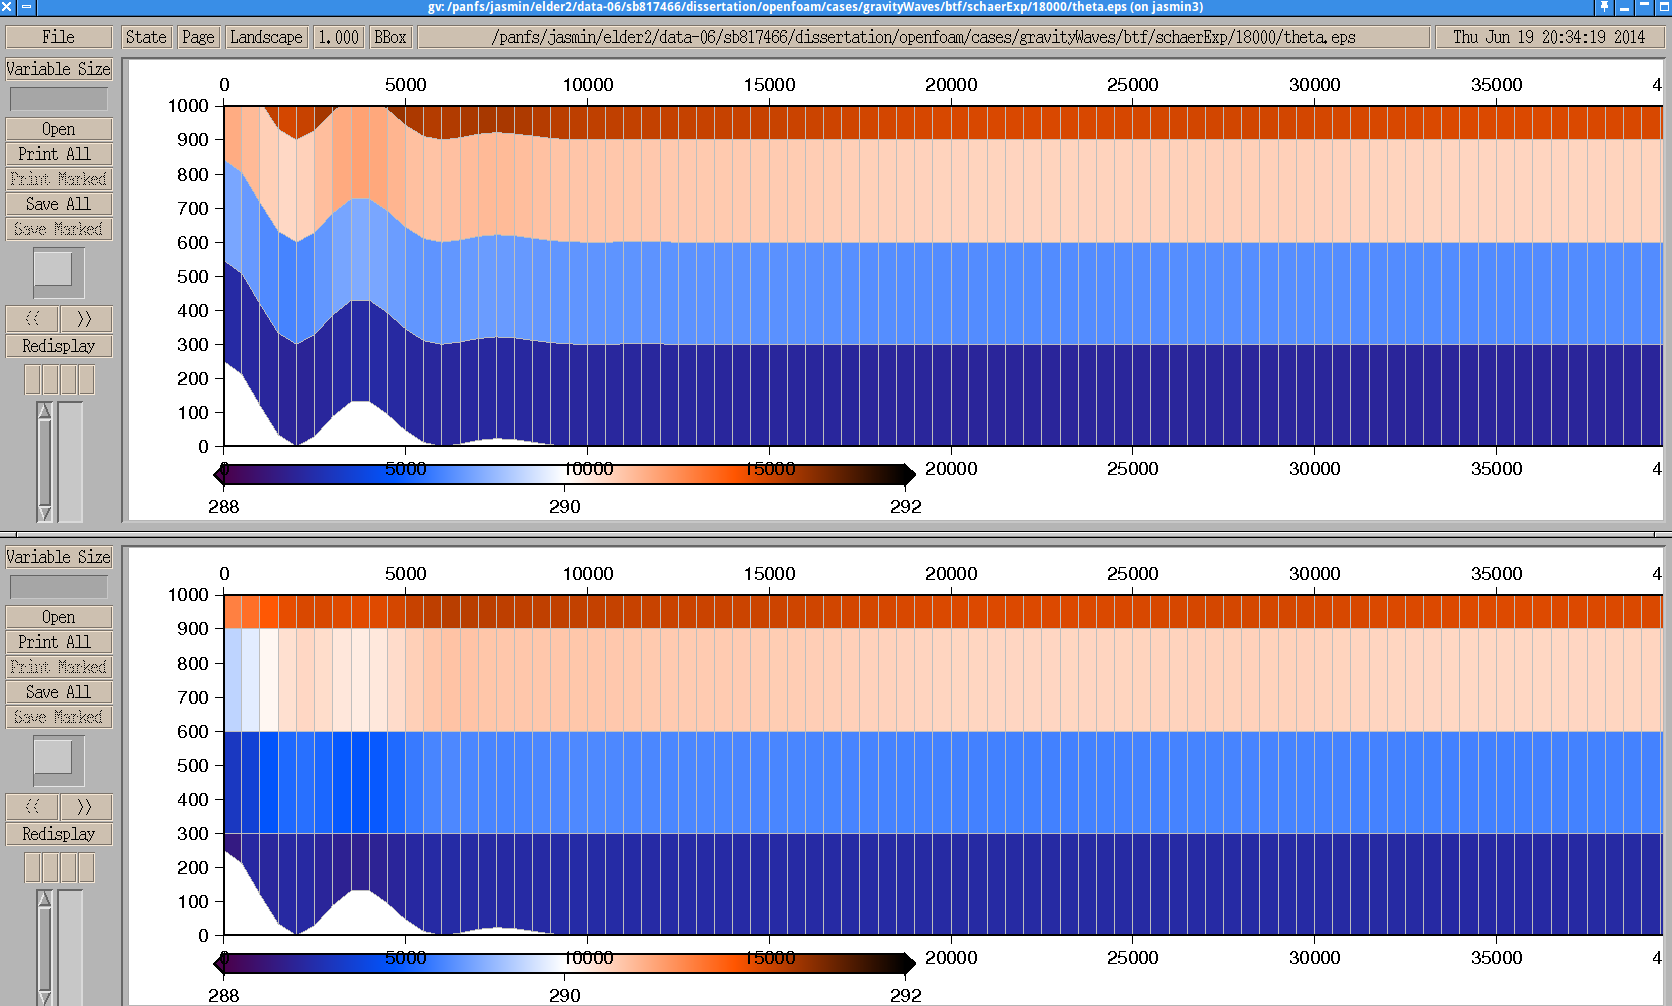
\includegraphics[width=\textwidth]{interim-results/gravityWavesBTFSnapColTheta.png}
	\caption{$\theta$ after t=18000s, BTF and SnapCol meshes}
	\label{fig:gw:theta}
\end{figure}

\begin{figure}
	BTF
	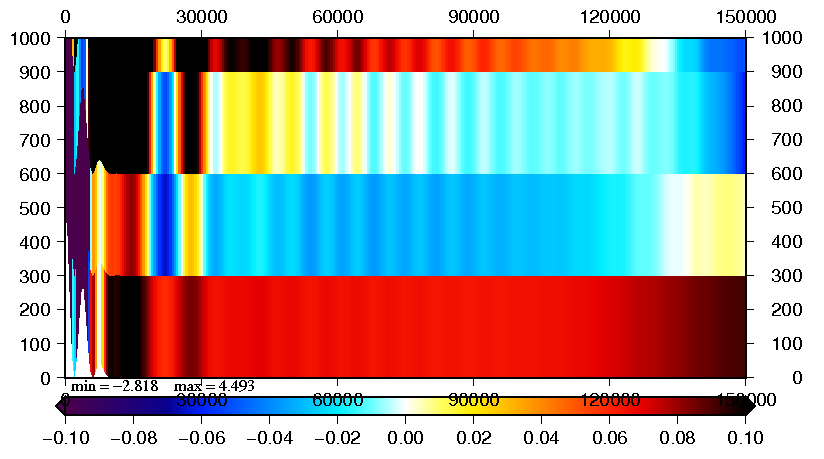
\includegraphics[width=\textwidth]{interim-results/gravityWavesBTFDoubleHeightThetaDiffZoom.png}
	SnapCol
	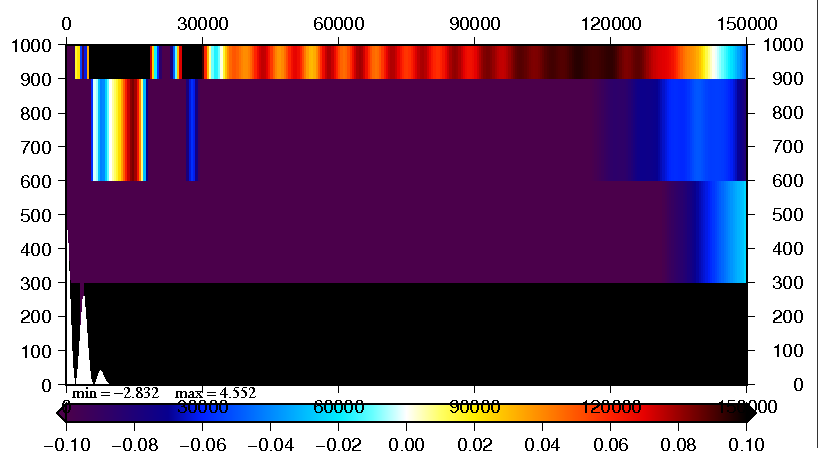
\includegraphics[width=\textwidth]{interim-results/gravityWavesSnapColDoubleHeightThetaDiffZoom.png}

	\caption{double height mountain, thetaDiff after t=18000s}
	\label{fig:gw:double-height}
\end{figure}

\begin{figure}
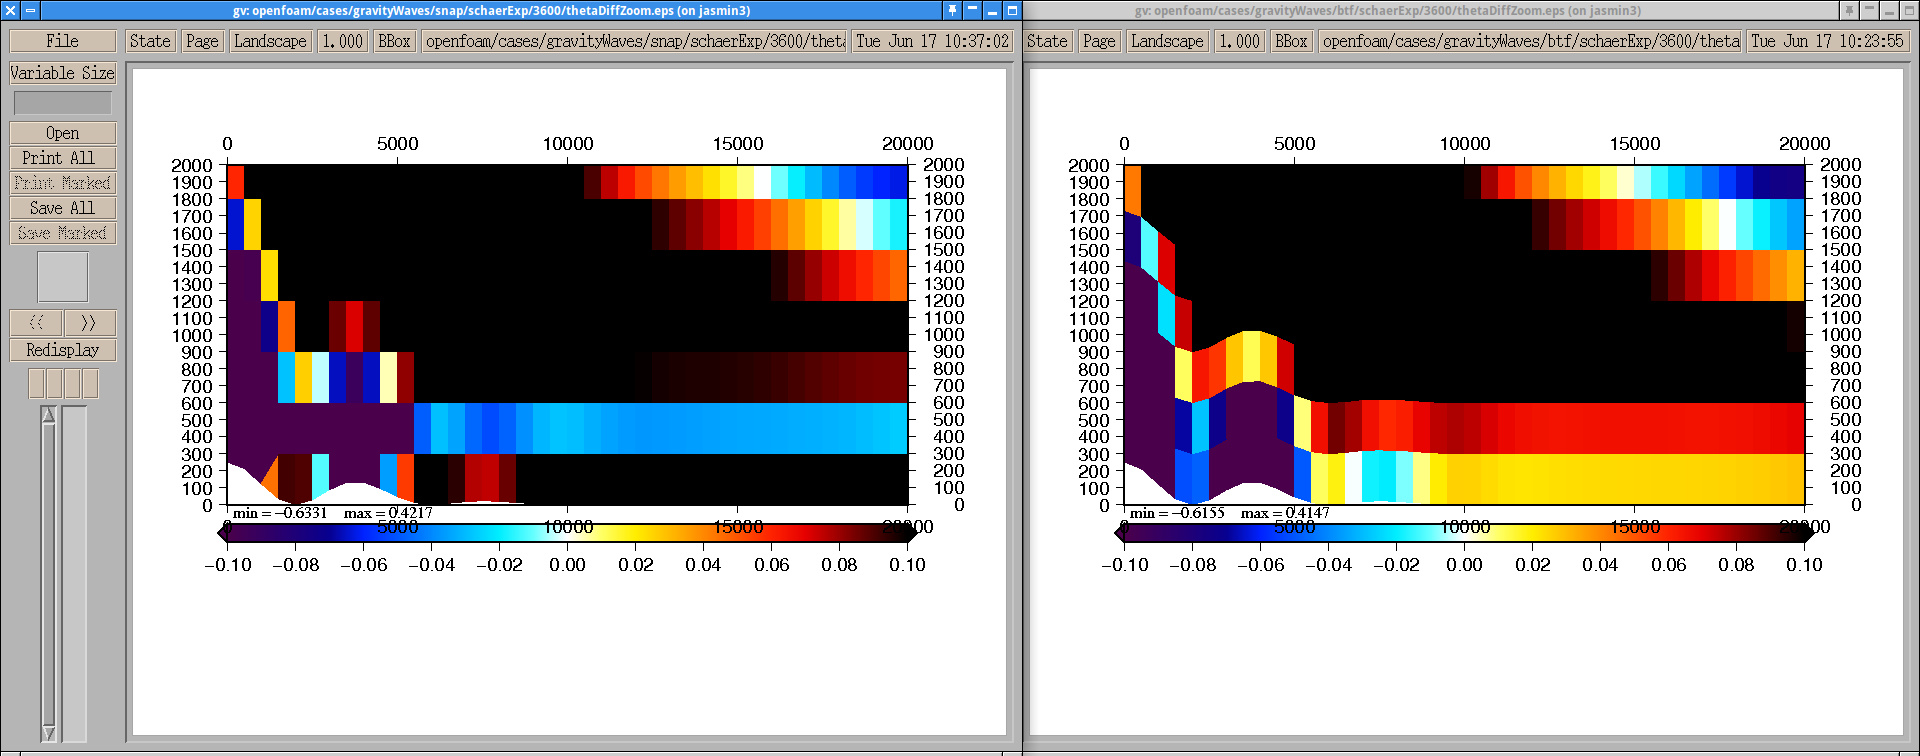
\includegraphics[width=\textwidth]{interim-results/gravityWavesBTFsnapMidZoom3600.png}
\caption{Vertical mixing after t=3600s, snap mesh left, BTF right}
\label{fig:gw:mixing-3600s}
\end{figure}

\begin{figure}
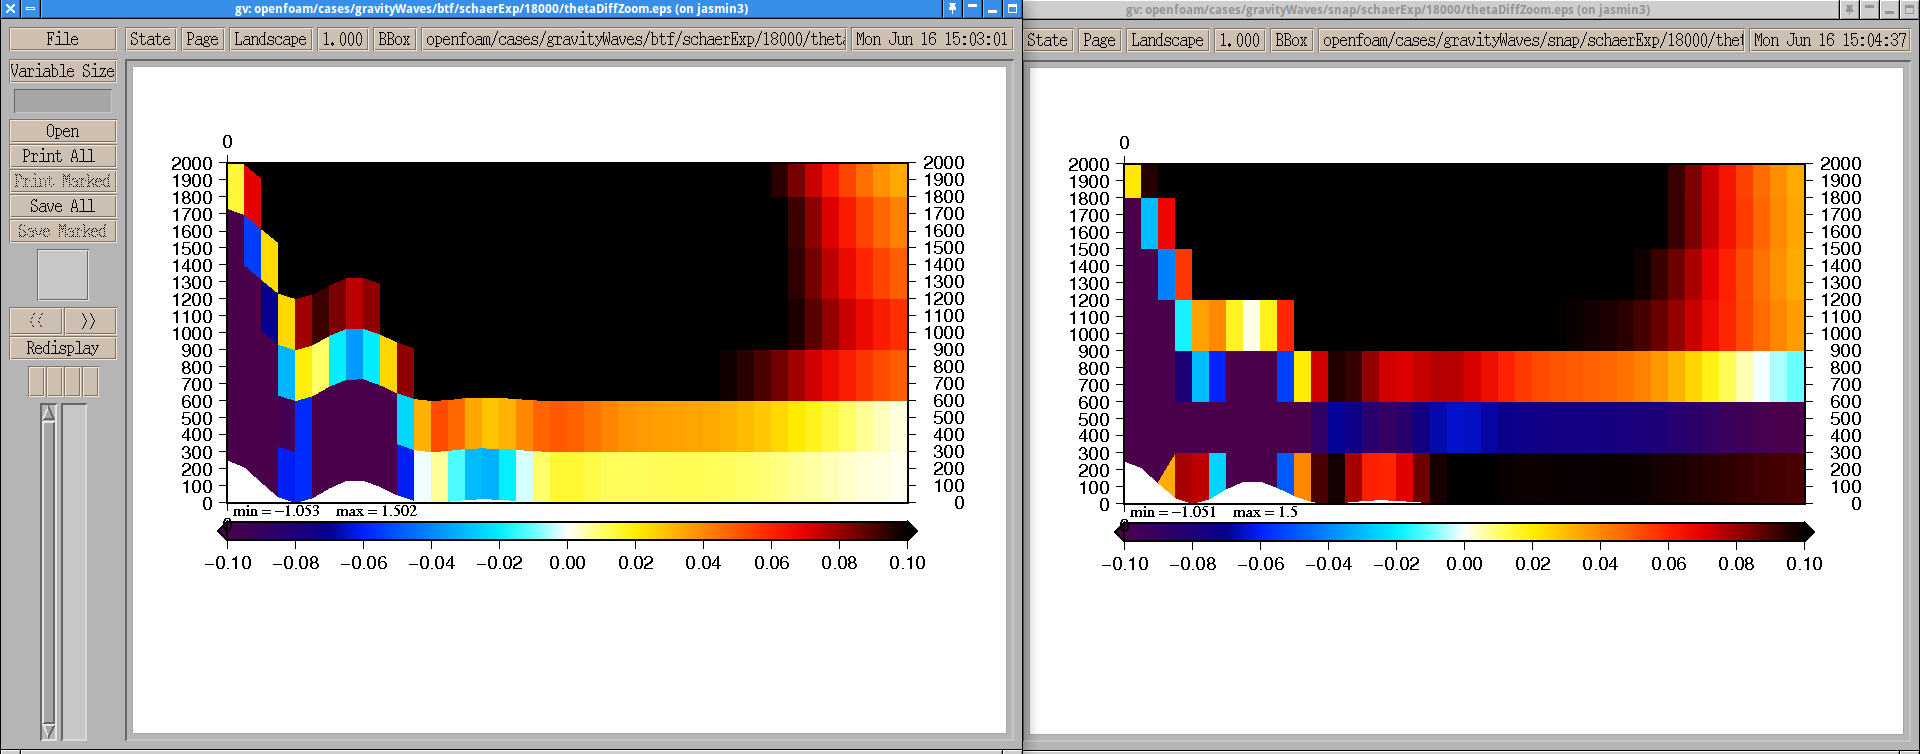
\includegraphics[width=\textwidth]{interim-results/gravityWavesBTFsnapMidZoom18000.png}
\caption{Vertical mixing after t=18000s.  Confusingly, snap mesh right, BTF left!}
\label{fig:gw:mixing-18000s}
\end{figure}

This suggests irreversible thermodynamic mixing (caused by numerical errors).  In reality, viscous effects would cause such mixing, but our equation set has no viscosity so there should be no mixing.

By isolating the nonlinear advection term in the momentum equations ($\del \rho \vect{u} \vect{u}$) we can see the different in flows between BTF and SnapCol meshes (Figure~\ref{fig:gw:nonlinear-advection}).  Looking at $U_f$ we can see larger velocities in small cells near mountain peaks, but otherwise flow fields are qualitatively in good agreement.

Noticing that $U_f$ follows the BTF mesh but does not follow the SnapCol mesh, we suspect that the thermal mixing may be caused by numerical diffusion (as we same with horizontal tracer advection).  This time, however, the flow is not horizontal, so it is SnapCol that has more diffusion.  To quantify this diffusion, we're going to measure entropy change.  We expect higher entropies where more mixing has occurred.  From Lauritzen and Thuburn 2012:

\begin{align}
	S &= - k_B \sum \theta \ln \theta \rho V
	\intertext{and, as a normalised change}
	\ell_s &= \frac{S - S^\mathrm{(initial)}}{S^\mathrm{(initial)}}
\end{align}
We could also compare with high resolution solution (coarse-grained), but Hilary hasn't got this working yet.  Adding an outlet sponge layer might help.

\subsection{Courant number}

\begin{itemize}
	\item Mean Courant numbers for cut-cell meshes and SLEVE are lower than BTF.  This could be because cells are relatively smaller aloft.
	\item Surprisingly, mean Courant number is slightly higher for snap mesh which has no small cells (Figure~\ref{fig:gw:courant}).
	\item SLEVE and BTF have the lowest max Co numbers, snap mesh significantly higher.  Since snap mesh does not have small cells, does this imply that snap mesh has higher winds?
\end{itemize}

Hilary mentioned that the reason that small cells aren't too much of a problem is that the small face is vertically oriented and has the majority of the flow fluxing through it.

\begin{align}
	\mathrm{Co} &= \frac{\Delta t}{2 V \rho} \sum{U}
	\intertext{where $U = \rho \vect{u} \cdot \vect{S}$ (ish.  see Eqn 6 in W\&S2014).  Given large near-horizontal surface $S_1$ and adjoining small vertical surface $S_2$}
	&= \frac{\Delta t}{2 S_1 S_2} \left( \vect{u} \cdot S_1 + \vect{u} \cdot S_2 \right)
	\intertext{which, when $S_2$ is sufficiently small}
	&\approx \frac{\Delta t}{2 S_1} \left( \vect{u} \cdot S_1 \right)
\end{align}
Hence, the Courant number is less affected by small cells with near-horizontal flow.

\begin{itemize}
	\item We can try increasing $\Delta t$ until SnapCol becomes unstable ($\mathrm{Co} > 1$), and compare results with TF meshes (and possibly Snap/SnapOrtho meshes) with the same timestep.  This will show that small cells are a problem.
	\item We could even try a sinking bubble test where the momentum will be fluxing through the large, almost-horizontally oriented face along the terrain surface
\end{itemize}

\begin{figure}
	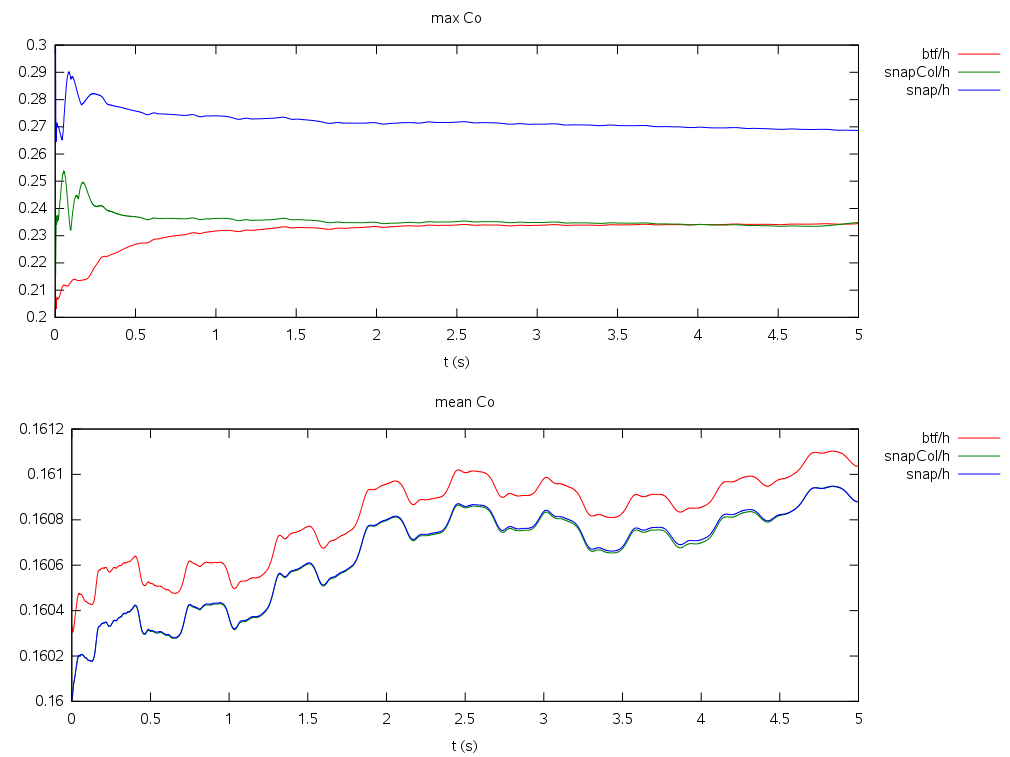
\includegraphics[width=\textwidth]{interim-results/gravityWavesCourants.png}
	\caption{Courant number for gravityWaves}
	\label{fig:gw:courant}
\end{figure}

\subsection{Energy}
\begin{itemize}
	\item Cut cell meshes are worse than TF meshes.  Snap loses internal energy much quicker than other meshes; i.e. it gets colder. (Figure~\ref{fig:gw:energy})
\end{itemize}

\begin{figure}
	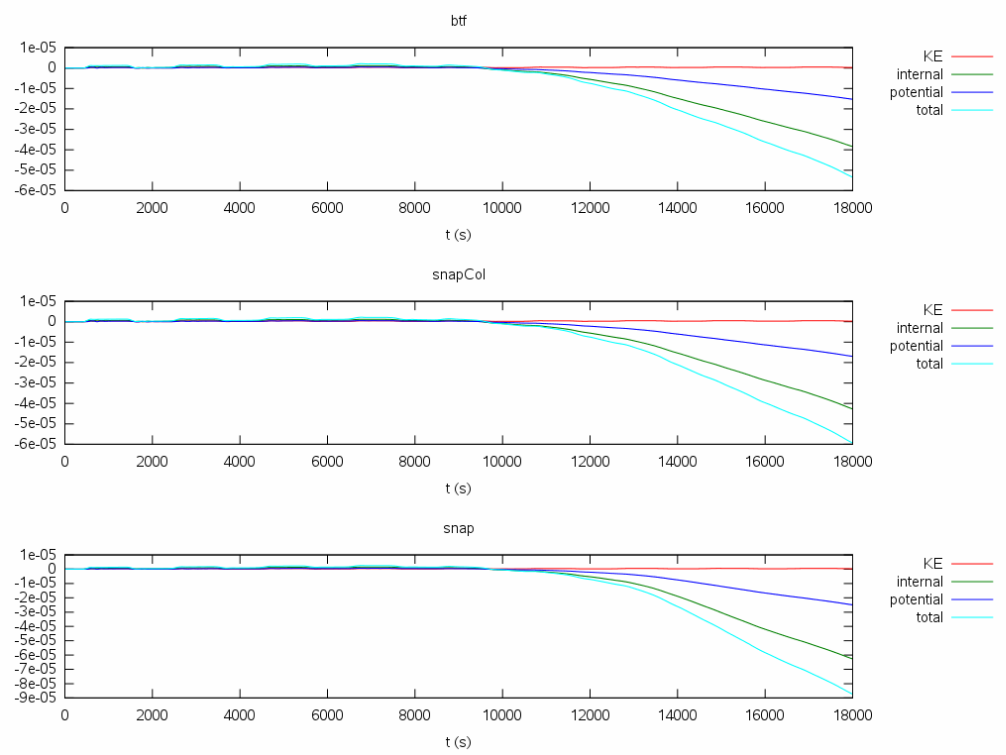
\includegraphics[width=\textwidth]{interim-results/gravityWavesEnergy.png}
	\caption{Energy changes}
	\label{fig:gw:energy}
\end{figure}

Looking at max Courant number for SLEVE, and energy loss graphs for all meshes, we see a change of behaviour at t=10000s (about 2.8 hours).  This might be related to gravity waves reflecting off the inlet or outlet boundary.  Changing the wind speed would let us investigate further.
